\documentclass[12pt]{article}

%% preamble: Keep it clean; only include those you need
\usepackage{amsmath}
\usepackage[margin = 1in]{geometry}
\usepackage{graphicx}
\usepackage{booktabs}
\usepackage{natbib}
% for space filling
\usepackage{lipsum}
% highlighting hyper links
\usepackage[colorlinks=true, citecolor=blue]{hyperref}

%% meta data

\title{Bridging Gaps: Investigating COVID-19's Influence on Health Disparities in Connecticut}
\author{Delia Lin\\
  Department of Statistics\\
  University of Connecticut
}

\begin{document}
\maketitle


\begin{abstract}
Here is the abstract.  
\end{abstract}


\section{Introduction}\label{sec:intro}

Use this section to answer three questions:
Why is the topic important/interesting?
What has been done on this topic in the literature?
What is your contribution?

\lipsum[1]

To cite a reference, here are examples. Textual:\citet{dwivedi2017analysis}. Parenthetical:\citep{xie2015dynamic}
\lipsum[2]

% roadmap
The rest of the paper is organized as follows.

The data will be presented in Section\ref{sec:data}

The methods are described in Section\ref{sec:meth}

The results are reported in Section\ref{sec:resu}

A discussion concludes in Section\ref{sec:disc}


\section{Data}\label{sec:data}

Use this section to describe the data that helps to answer your research
questions. In display equation 1:
\begin{equation}\label{eq:mc2} 
  E = m c^2,
\end{equation}
which states that the energy $E$ of a particle in its rest frame as the product
of mass ($m$) with the speed of light squared ($c^2$). In line equation: $E=m c^2$~\ref{eq:mc2}
\lipsum{1}

\section{Methods}\label{sec:meth}

Use this section to present the methodologies that will generate results by
analyzing the data. In display equation 2: 
\begin{equation}
  \label{eq:area}
  \pi r^2.
\end{equation}

Equation\ref{eq:area} is interesting. In line equation: $\pi r^2$.\lipsum[1]

Sometimes I don't want an equation to be numbered such as this one:
\[
  f(x) = \frac{1}{\sqrt{2\pi}} \exp\left( - \frac{x^2}{2} \right),
\]
which is the density of a standard normal variable.



\section{Results}\label{sec:resu}


Table\ref{tab:rv} summarizes some example draws from some distributions.
\lipsum[1]

\begin{table}[tbp]
  \caption{This is my first table.}\label{tab:rv}
\centering
\begin{tabular}{rrr}
  \toprule
  \begin{table}[]
    \begin{tabular}{lllllllllll}
    \textbf{COUNTY}                                         &                                              & Fairfield County & Hartford County & Litchfield County & Middlesex County & New Haven County & New London County & Tolland County & Windham County &  \\
    \textbf{Total Population}                               &                                              & 944977           & 894465.25       & 182657.5          & 163318.25        & 858678           & 268477.75         & 151218.75      & 116608.75      &  \\
    \textbf{RACE}                                           & American Indian and Alaska Native race alone & 0.24             & 0.3075          & 0.2025            & 0.195            & 0.1725           & 0.605             & 0.05           & 0.565          &  \\
                                                            & Asian                                        & 5.2925           & 5.2925          & 1.9               & 3.0625           & 4.005            & 4.12              & 4.675          & 1.3675         &  \\
                                                            & Black or African American                    & 11.405           & 13.7025         & 1.83              & 5.385            & 13.34            & 5.8175            & 3.1075         & 2.33           &  \\
                                                            & Native Hawaiian and Pacific Islander         & 0.055            & 0.035           & 0                 & 0.005            & 0.0225           & 0.025             & 0              & 0.015          &  \\
                                                            & White                                        & 72.6325          & 70.67           & 92.6025           & 88.0875          & 73.2875          & 80.6175           & 88.025         & 88.8725        &  \\
    \textbf{Ethnicity}                                      & Hispanic                                     & 19.53            & 17.8275         & 6.15              & 6.12             & 17.885           & 10.5              & 5.4475         & 11.6375        &  \\
    \textbf{Average rehospitalization rate   in the county} &                                              & 0.1575           & 0.14            & 0.145             & 0.1325           & 0.16             & 0.14              & 0.14           & 0.1375         &  \\
    \textbf{Education}                                      & Associates                                   & 20.74            & 25              & 27.9225           & 26.46            & 24.4175          & 29.2675           & 26.315         & 30.9775        &  \\
                                                            & Bachelor                                     & 26.53            & 21.4575         & 20.635            & 23.3325          & 18.785           & 18.3175           & 23.4075        & 14.595         &  \\
                                                            & Graduate Degree                              & 21.14            & 16.475          & 14.6975           & 18.4525          & 16.3425          & 15.18             & 17.865         & 9.55           &  \\
                                                            & HS Graduate                                  & 21.4725          & 26.7175         & 29.5875           & 26.0275          & 30.565           & 29.46             & 27.03          & 33.5125        &  \\
                                                            & Less the High School                         & 10.12            & 10.3525         & 7.1575            & 5.7275           & 9.8875           & 7.7725            & 5.385          & 11.365         & 
    \end{tabular}
    \end{table}
   \bottomrule
\end{tabular}
\end{table}

Figure\ref{fig:cars} shows the distance against the speed from this dataset.
\begin{figure}[tbp]
  \centering
  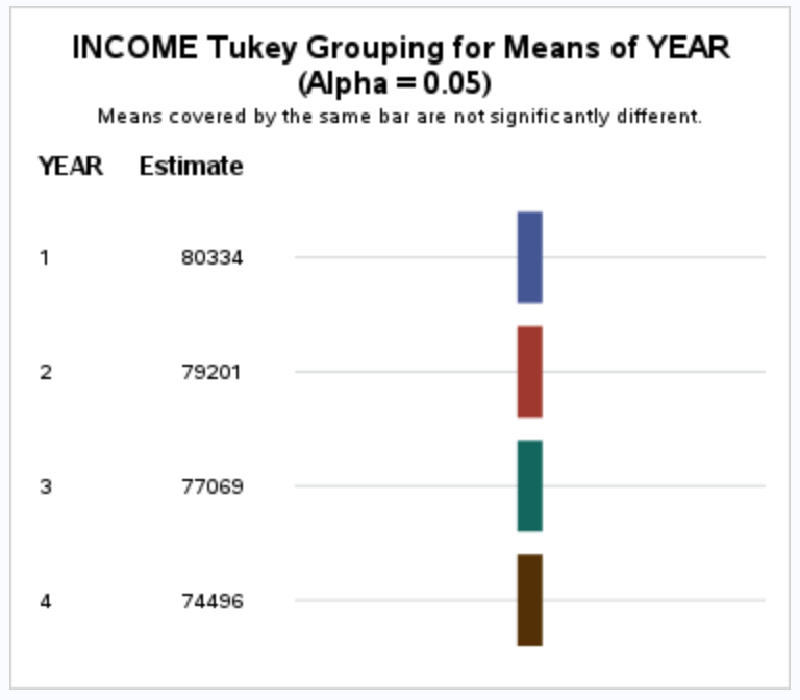
\includegraphics[width=\textwidth]{Income by year.pdf}
  \caption{This is my first figure.}\label{fig:cars}
\end{figure}

\section{Discussion}\label{sec:disc}

What are the main contributions again?

What are the limitations of this study?

What are worth pursuing further in the future?

\lipsum[1]
Watch for prevalence of diabetes \citep{wild2004global}.
\citet{wild2004global}

\appendix

\bibliography{refs}
\bibliographystyle{mcap}

\end{document}